%+----------------------------------------------------------------------------+
%| SLIDES: 
%| Chapter: Configuration Space
%| Author: Antonio miti
%| Event: Phd Colloquium - What is ... Geometric mechanics?
%+----------------------------------------------------------------------------+

%- HandOut Flag -----------------------------------------------------------------------------------------
\makeatletter
\@ifundefined{ifHandout}{%
  \expandafter\newif\csname ifHandout\endcsname
}{}
\makeatother

%- D0cum3nt ----------------------------------------------------------------------------------------------
\documentclass[beamer,10pt]{standalone}   
%\documentclass[beamer,10pt,handout]{standalone}  \Handouttrue  

\ifHandout
	\setbeameroption{show notes} %print notes   
\fi

	
%- Packages ----------------------------------------------------------------------------------------------
\usepackage{custom-style}
\usetikzlibrary{positioning}
\usepackage{multicol}


%--Beamer Style-----------------------------------------------------------------------------------------------
\usetheme{toninus}
\usepackage{animate}
\usetikzlibrary{positioning, arrows}
\usetikzlibrary{shapes}

\begin{document}
%-------------------------------------------------------------------------------------------------------------------------------------------------
\begin{frame}{Phase Space via Configuration Space}
	\begin{itemize}
	\item To introduce the notion of {\bf phase space} it is useful to start from the auxiliary concept of {\bf configuration space}.
	\end{itemize}

	\vfill
	\begin{itemize}
		\item<2-> this notion is based on three \emph{primitive concepts}:
	\end{itemize}
	\onslide<2->{
		\begin{center}
			\begin{tikzpicture}[>=stealth,every node/.style={shape=rectangle,draw,rounded corners},node distance=0.05\linewidth,]
		    % create the nodes
			    \node[] (a1) {Ambient (space)}; %Physical space
			    \node[] (a2)[right =of a1] {Body}; %(Physical) system
			    \node[] (a3)[right =of a2] {Displacement}; %configuration
			\end{tikzpicture}
		\end{center}
	}
\end{frame}
\note[itemize]{
\item an elementary way for introducing the notion of phase space starts from the concept of \emph{configuration space}.
\item this is in turn based on three first principles: Space, Body, Displacement.
\item they cannot be defined in a strict sense but one can provide intuition and a mathematical realization.

\item
In many presentations of mathematical notions by primitive concept or primitive notion is meant a concept which, due to its simplicity and intuitiveness, one renounces to define by means of terms and concepts already defined within a formal system, and which on the contrary is chosen to exploit to formulate the definition of other concepts; therefore a primitive concept is accepted without explanation because its meaning is obvious or self-evident.
}
%-------------------------------------------------------------------------------------------------------------------------------------------------


%-------------------------------------------------------------------------------------------------------------------------------------------------
\begin{frame}[t]{Configuration Space: the Ambient}
	\begin{center}
		\begin{tikzpicture}[>=stealth,every node/.style={shape=rectangle,draw,rounded corners},node distance=0.05\linewidth,]
	    % create the nodes
		    \node[red] (a1) {Ambient (space)}; %Physical space
		    \node[gray] (a2)[right =of a1] {Body}; %(Physical) system
		    \node[gray] (a3)[right =of a2] {Displacement}; %configuration
		\end{tikzpicture}	
	\end{center}
	\begin{columns}
		\begin{column}[T]{0.5\textwidth}
			\begin{itemize}
				\item The physical space, our universe.
				\item It is the stage on which the act of dynamics takes place.
			\end{itemize}
			\vspace{1em}
			\onslide<2->{					
				\begin{exblock}
					Consider a laboratory.
				\end{exblock}
			}
			\vspace{1em}
			\onslide<3->{
				\begin{mathblock}
					is the Euclidean space $E=\mathbb{R}^3$.
					\\				
					(fixed a \emph{Galilean observer}) 
				\end{mathblock}
			}		
		\end{column}
		\begin{column}[T]{0.5\textwidth}
			\onslide<2->{
				\begin{center}
					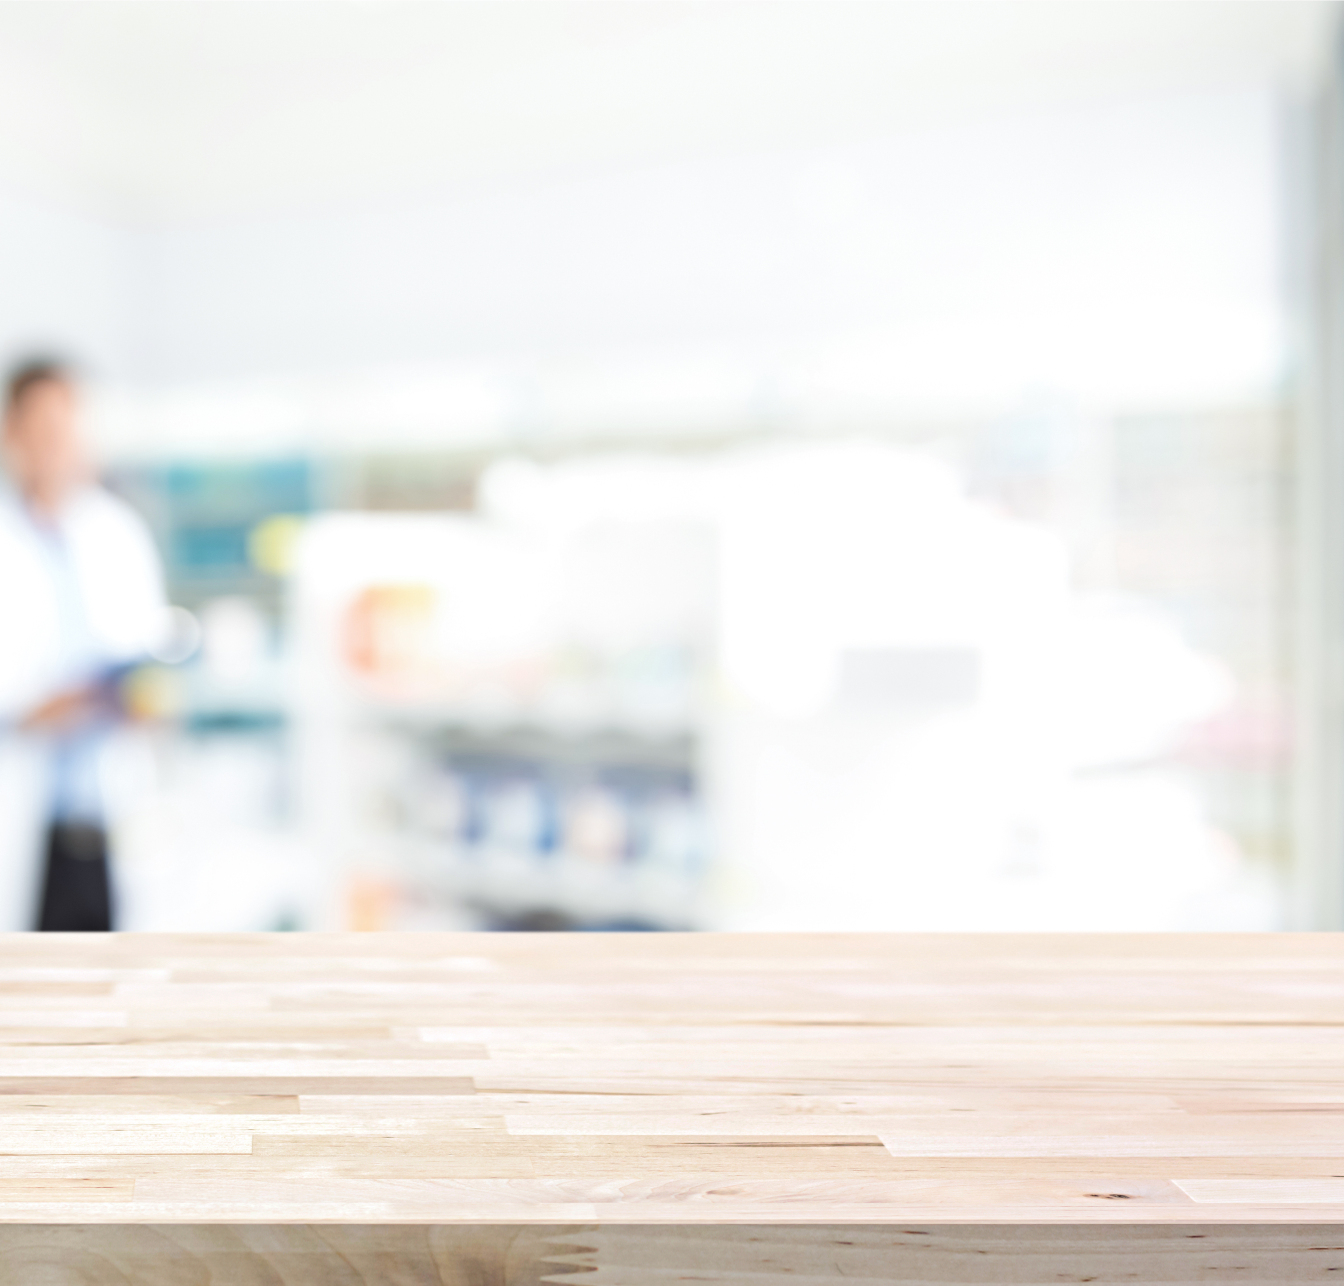
\includegraphics[width=\textwidth]{Pictures/emptylab}
				\end{center}
			}
		\end{column}
	\end{columns}
\end{frame}
\note[itemize]{
	\item
}
%-------------------------------------------------------------------------------------------------------------------------------------------------


%-------------------------------------------------------------------------------------------------------------------------------------------------
\begin{frame}[t]{Configuration Space: the Body}
	\begin{center}
		\begin{tikzpicture}[>=stealth,every node/.style={shape=rectangle,draw,rounded corners},node distance=0.05\linewidth,]
	    % create the nodes
		    \node[gray] (a1) {Ambient (space)}; %Physical space
		    \node[red] (a2)[right =of a1] {Body}; %(Physical) system
		    \node[gray] (a3)[right =of a2] {Displacement}; %configuration
		\end{tikzpicture}
	\end{center}

	\begin{columns}
		\begin{column}[T]{0.5\textwidth}
			\begin{itemize}
				\item it is a bulk of matter, a portion of the ambient, we wish to study.
			\end{itemize}
								
			\vspace{1em}
			\only<2->{			
				\begin{exblock}
					Consider the bob of a rigid pendulum.
				\end{exblock}
			}

			\vspace{1em}
			\only<3->{
				\begin{mathblock}
					\begin{columns}
						\begin{column}{0.025\textwidth}
						\end{column}
						\begin{column}[T]{0.5\textwidth}
							is a submanifold $B\hookrightarrow E$ with boundary
							\vspace{-.5em}
							\begin{center}
								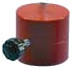
\includegraphics[width=.25\textwidth]{Pictures/bob}
							\end{center}
						\end{column}					
						\begin{column}[T]{0.45\textwidth}
							is a point in $B\in E$ (the center of mass).
							\begin{center}
								\tikz[] \node[scale=0.5,coordinate,fill=red,circle] (n1) {};	
							\end{center}						
						\end{column}							
					\end{columns}
					\begin{column}{0.025\textwidth}
					\end{column}
				\end{mathblock}
			}
			\vfill
%			\only<4->{
%				\begin{bracketbox}%{Key point:}
%					\small
%					Remind:
%					The ambient acts on the body via \emph{forces} and \emph{constraints}.
%				\end{bracketbox}
%			}	
		\end{column}
		\begin{column}[T]{0.5\textwidth}
				\begin{center}
					\ifHandout \else
						\includegraphics<1>[width=\textwidth]{Pictures/emptylab}
					\fi
					\includegraphics<2->[width=\textwidth]{Pictures/Pendolab}					
				\end{center}
		\end{column}
	\end{columns}
\end{frame}
\note[itemize]{
	\item "The body is the protagonist of the act" (Ambient is the stage)
	\item remind the implied idea: 	The ambient acts on the body via \emph{forces} and \emph{constraints}.
}	
%-------------------------------------------------------------------------------------------------------------------------------------------------


%-------------------------------------------------------------------------------------------------------------------------------------------------
\begin{frame}[t]{Configuration Space: the displacement}
	\begin{center}
		\begin{tikzpicture}[>=stealth,every node/.style={shape=rectangle,draw,rounded corners},node distance=0.05\linewidth,]
	    % create the nodes
		    \node[gray] (a1) {Ambient (space)}; %Physical space
		    \node[gray] (a2)[right =of a1] {Body}; %(Physical) system
		    \node[red] (a3)[right =of a2] {Displacement}; %configuration
		\end{tikzpicture}
	\end{center}

	\begin{columns}
		\begin{column}[T]{0.5\textwidth}
			\begin{itemize}
				\item is how the body is placed inside the space.
				\item configuration (spatial displacement) of the physical system admissible by the constraints.
			\end{itemize}
			\vspace{1em}
			\only<2->{
				\begin{exblock}[Pendulum]
					one of the possible positions where the bob can be placed allowed by the rod.		
				\end{exblock}
			}	
			\vspace{1em}
			\only<3->{
				\begin{mathblock}
					is a (smooth) function $B \to E$.				
				\end{mathblock}
			}					
			
		\end{column}
		\begin{column}[T]{0.5\textwidth}
			\begin{center}
				\ifHandout \else
					\includegraphics<1>[width=\textwidth]{Pictures/Pendolab}
				\fi				
				\only<2->{	
					\animategraphics[autoplay,palindrome,width=\textwidth]{5}{Pictures/pendolum-frame/pendo}{1}{9}
				}
			\end{center}
		\end{column}
	\end{columns}
\end{frame}
\note[itemize]{
	\item
}

%-------------------------------------------------------------------------------------------------------------------------------------------------

%-------------------------------------------------------------------------------------------------------------------------------------------------
\begin{frame}[t]{Configuration Space}
	%	
	\center
	\begin{zigzagbox}
		Neglect the fluff $\quad\rightsquigarrow\quad$ abstract (synthetic) mathematical setting
	\end{zigzagbox}
	
	\begin{columns}
		\begin{column}[T]{0.5\textwidth}
			\begin{itemize}
				\item<2-> Consider the set $Q$  of all the possible displacements (spatial configurations).
			\end{itemize}
			%			
			\vspace{1em}
			\onslide<3->{
				\begin{exblock}[Pendulum]
					$Q$ = 
						the locus of points on the plane with fixed distance from the pivot (the circle $S^1$).	
				\end{exblock}
			
			}			
			%			
			\vspace{1em}
			\onslide<4->{
				\alert{Upshot: $Q$ is a smooth manifold}
							
			\begin{defblock}[Configuration Space]
				Smooth manifold of all the system configurations admissible by the constraints.
			\end{defblock}			
			}
		\end{column}


		\begin{column}[T]{0.5\textwidth}
			\begin{center}
			\only<1>{				
				\resizebox{\textwidth}{!}{		
				    \begin{tikzpicture}
					    %frame
					    \draw[draw=none] (-5,-8) rectangle (5,5);
						% Support
						\coordinate (o) at (0,0);
						\node[cross out,draw,black!10] (0,0){};
						\node[circle,draw,black!10] (0,0){};
						% Bob's trajectory
						\draw[blue,line width=1mm,] (0,0) circle (4);
						% Rod + Bob
						\draw[dashed] (0,0) -- (-60:4) node[fill,circle,red](m){};
				    \end{tikzpicture}
				}
			}
			\only<2->{				
				\resizebox{\textwidth}{!}{		
					\pgfmathtruncatemacro\steps{50}
					\pgfmathtruncatemacro\maxtheta{30}
					\pgfmathtruncatemacro\pi{3.14}
					\begin{animateinline}[autoplay,loop]{10} % 5 fps, same as 0.2 s transduration
					  \multiframe{\steps}{i=0+1}{
					    \begin{tikzpicture}
					    \pgfmathsetmacro\fraction{\i/(\steps-1)}
						\pgfmathsetmacro\theta{\maxtheta*cos(360*\fraction)-90}
					    %frame
					    \draw[draw=none] (-5,-8) rectangle (5,5);
						% Support
						\coordinate (o) at (0,0);
						\node[cross out,draw,black!10] (0,0){};
						\node[circle,draw,black!10] (0,0){};
						% Bob's trajectory
						\draw[blue,line width=1mm] (0,0) circle (4);
						% Rod + Bob
						\draw[dashed] (0,0) -- (\theta:4) node[fill,circle,red](m){};
					    \end{tikzpicture}
					  }
					\end{animateinline}
				}
			}
			\end{center}
		\end{column}
	\end{columns}
\end{frame}
\note[itemize]{
	\item Neglect the fluff in the wording of Galilei:
		\\
    Adunque, tuttalvolta che in concreto voi applicate una sfera materiale a un piano materiale, voi applicate una sfera non perfetta a un piano non perfetto; e questi dite che non si toccano in un punto. Ma io vi dico che anco in astratto una sfera immateriale, che non sia sfera perfetta, può toccare un piano immateriale, che non sia piano perfetto, non in un punto, ma con parte della sua superficie; talché sin qui quello che accade in concreto, accade nell'istesso modo in astratto: e sarebbe ben nuova cosa che i computi e le ragioni fatte in numeri astratti, non rispondessero poi alle monete d'oro e d'argento e alle mercanzie in concreto. Ma sapete, signor Simplicio, quel che accade? Sì come a voler che i calcoli tornino sopra i zuccheri, le sete e le lane, bisogna che il computista faccia le sue tare di casse, invoglie ed altre bagaglie, così, quando il filosofo geometra vuol riconoscere in concreto gli effetti dimostrati in astratto, bisogna che difalchi gli impedimenti della materia; che se ciò saprà fare io vi assicuro che le cose si riscontreranno non meno aggiustatamente che i computi aritmetica Gli errori dunque non consistono né nell'astratto né nel concreto, né nella geometria o nella fisica, ma nel calcolatore, che non sa fare i conti giusti. (G. Galilei, Dialogo sopra i due massimi sistemi, tolemaico e copernicano, a cura di Libero Sosio, Einaudi, Torino, p. 252).
}
%-------------------------------------------------------------------------------------------------------------------------------------------------

%-------------------------------------------------------------------------------------------------------------------------------------------------
\begin{frame}{Quick reminder: Smooth manifolds}
	\tcbset{colback=white,
	colbacktitle=white,
	colframe=red!70!black,
	boxrule=1pt,
	colupper=red!70!black,
	arc=15pt,
	}
		\begin{columns}[]
		\begin{column}{0.475\textwidth}
			\begin{tcolorbox}[enhanced,frame hidden,borderline={0.5pt}{0pt}{red!70!black}]
			Extrinsically:\\
			\color{black} 
			\emph{higher dimensional} surface 
			\\ smoothly embedded in $\mathbb{R}^N$.
			\\
			\small (for a suitably large $N$).		
			\end{tcolorbox}
	
			\center
			\onslide<2->{
				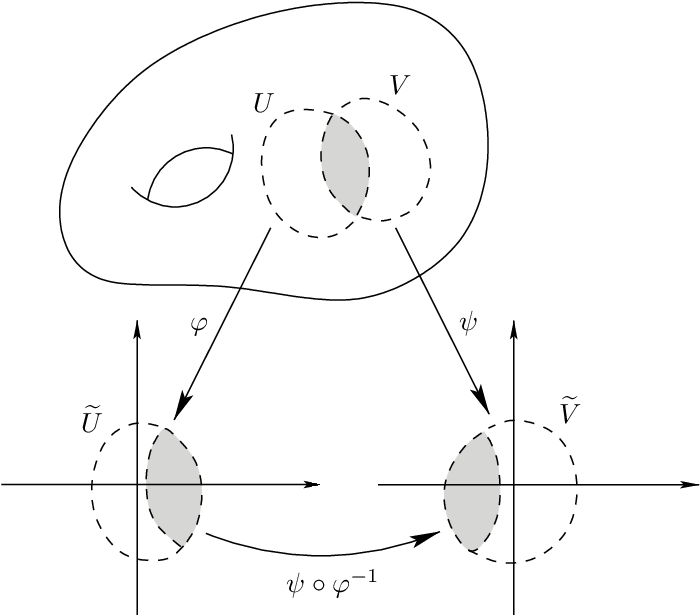
\includegraphics[width=.9\textwidth, height = 10em]{Pictures/smooth-mfd-Lee} 	
				%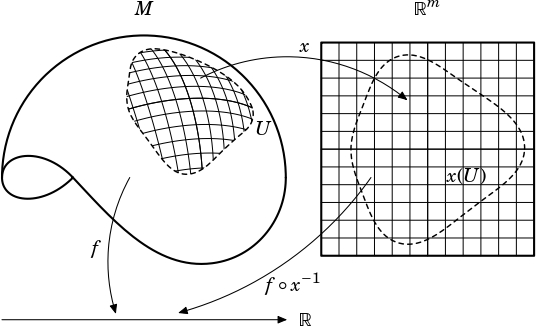
\includegraphics[width=.7\textwidth]{Pictures/LocalChart} 		
			}
		\end{column}
		\begin{column}{0.52\textwidth}
			\center
			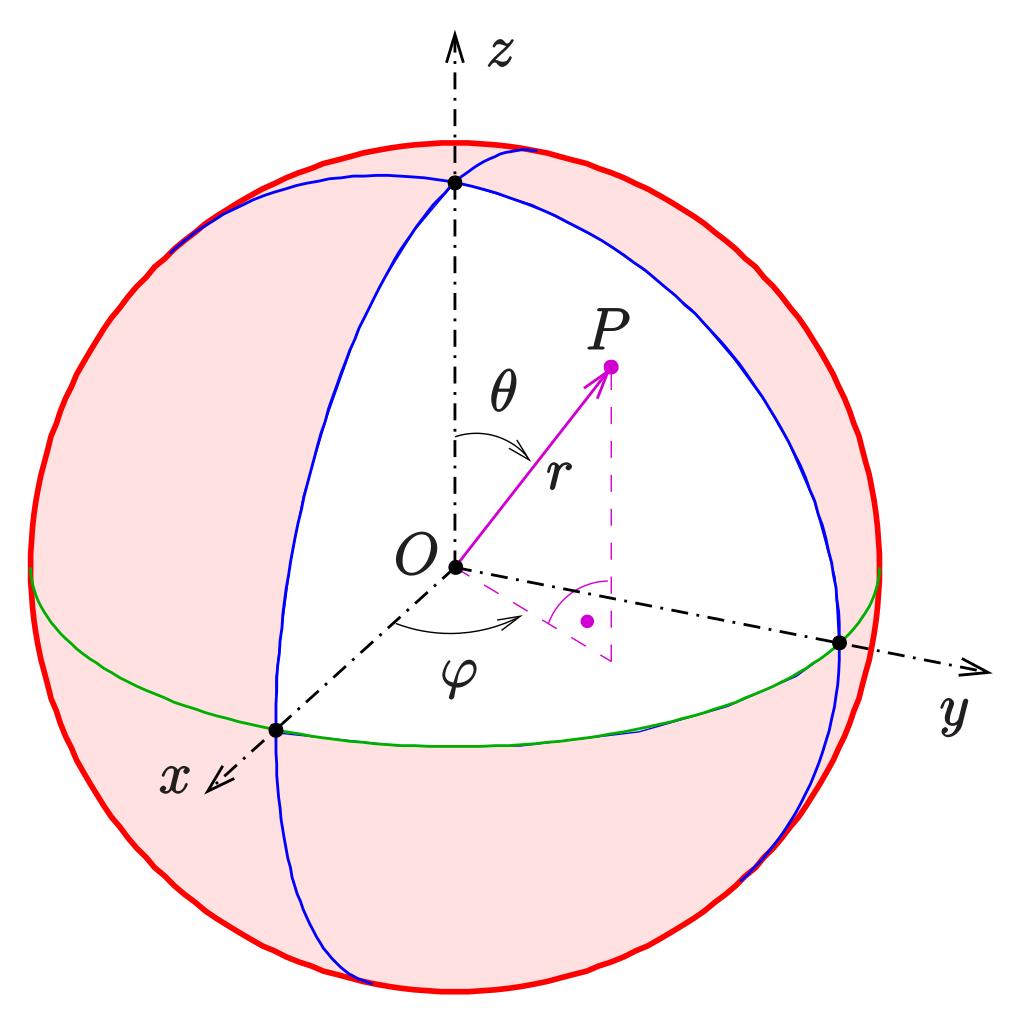
\includegraphics[width=.5\textwidth]{Pictures/embedded_sphere} 	
			
			\onslide<2->{
				\begin{tcolorbox}[enhanced,frame hidden,borderline={0.5pt}{0pt}{red!70!black}]
					Intrinsically:\\
					\color{black} 
					A topological spaces equipped with 
					\\ (a maximal atlas of compatible) 
					\\
					charts.
				\end{tcolorbox}			
			}			
		\end{column}
		\end{columns}
		
		\vfill
		\begin{columns}[]
			\begin{column}{0.1\textwidth}\end{column}
			\begin{column}{0.6\textwidth}
				\onslide<3->{
			\begin{tcolorbox}[enhanced,frame hidden,borderline={0.5pt}{0pt}{brown!70!black}]
				A reasonably general setting for defining:
				\begin{itemize}
					\item[•] Reference frames / coordinates (observers);
					\item[•] Smoothness.
				\end{itemize}
			\end{tcolorbox}
				}
			\end{column}
			\begin{column}{0.1\textwidth}\end{column}
		\end{columns}






\end{frame}
\note[itemize]{
	\item The sphere centered in the origin of the Cartesian space is a prototypical example.
	\item Intrinsically, smoothness is encoded requiring the property that transition functions on overlapping charts are smooth.
}
%-------------------------------------------------------------------------------------------------------------------------------------------------


%-------------------------------------------------------------------------------------------------------------------------------------------------
\ifHandout
\begin{frame}[t]{Configuration Space: a slightly more difficult example}

		\begin{columns}[T]
			\begin{column}{0.5\textwidth}
				\center
				\begin{bracketbox}
					Double pendulum.
				\end{bracketbox}
			\end{column}
			\begin{column}{0.5\textwidth}
				\noindent Toy model for:
				\begin{columns}
					\begin{column}{0.5\textwidth}
						\begin{center}
							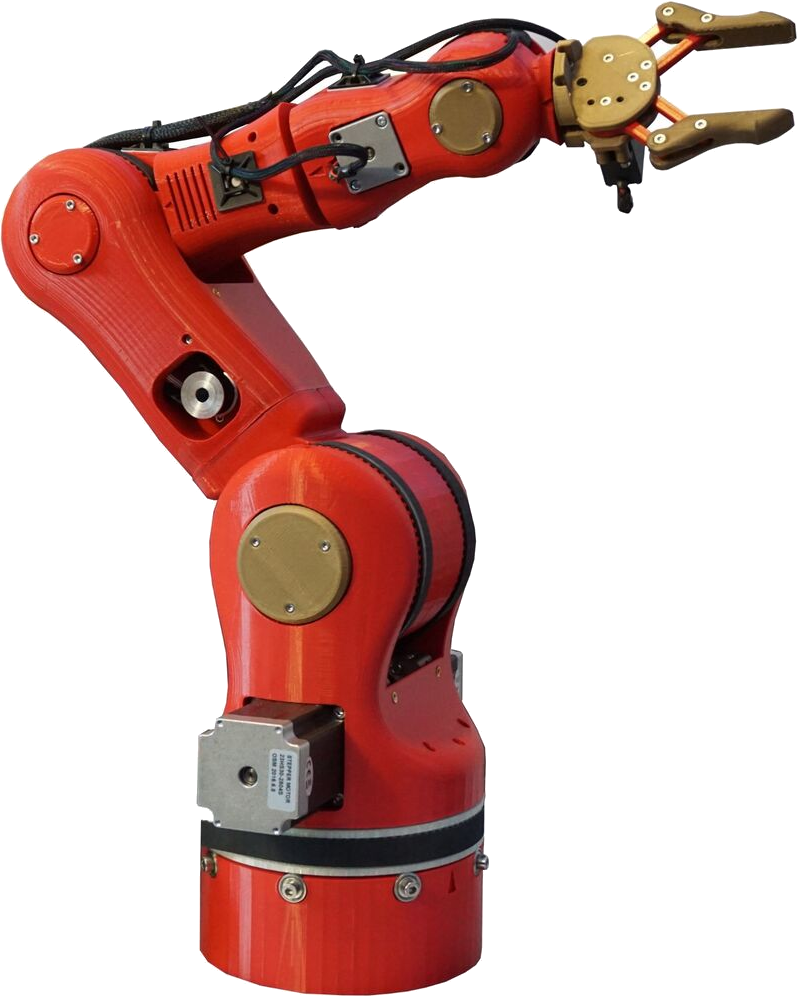
\includegraphics[width=.55\textwidth]{Pictures/robo_arm}	
						\end{center}
						mechanical arms.
					\end{column}			
					\begin{column}{0.5\textwidth}
						\begin{center}
							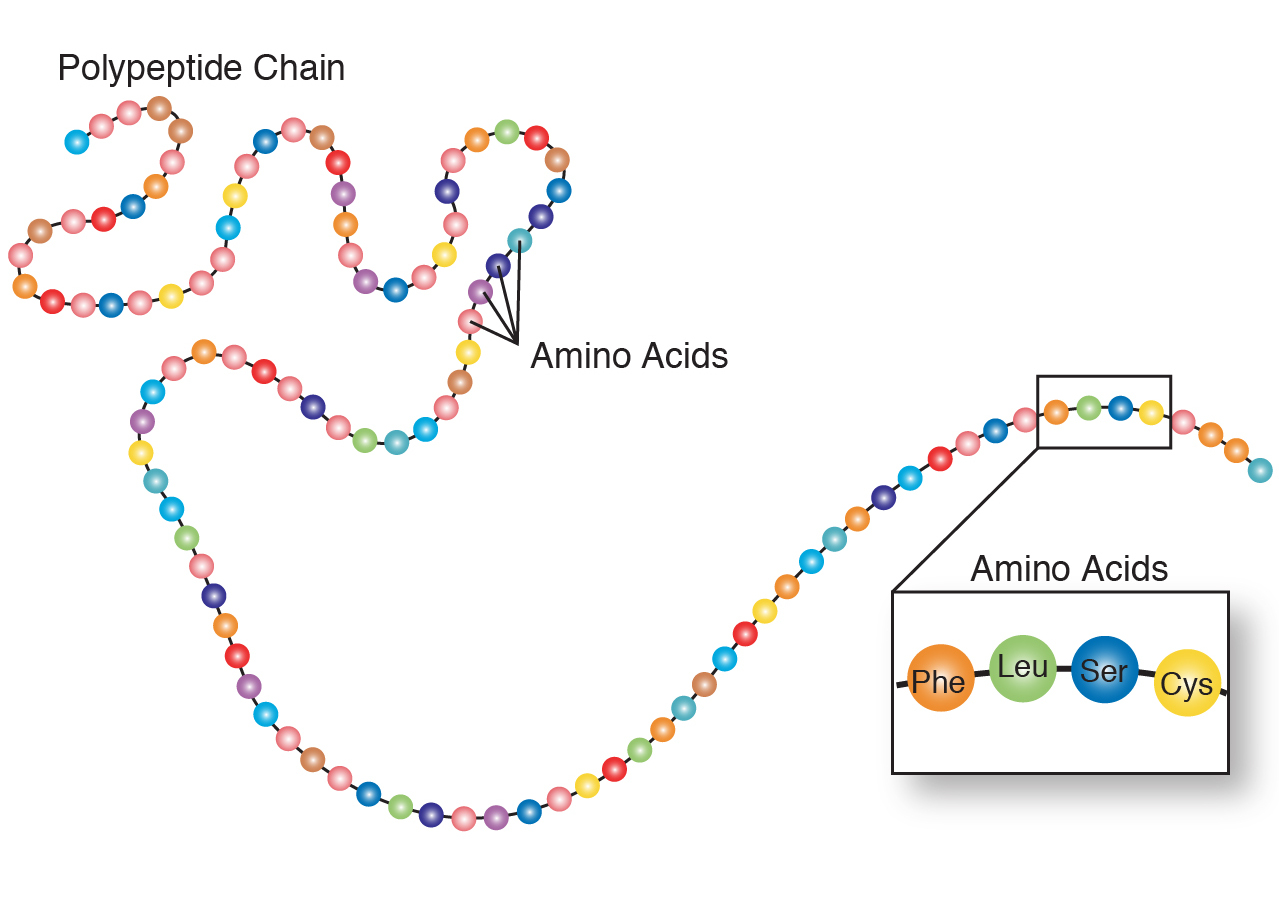
\includegraphics[width=.65\textwidth]{Pictures/amino_acids}
						\end{center}
						Proteins (amino acid chains).
					\end{column}				
				\end{columns}
			\end{column}				
		\end{columns}


		\begin{columns}[T]
			\begin{column}{0.5\textwidth}
				\begin{center}
					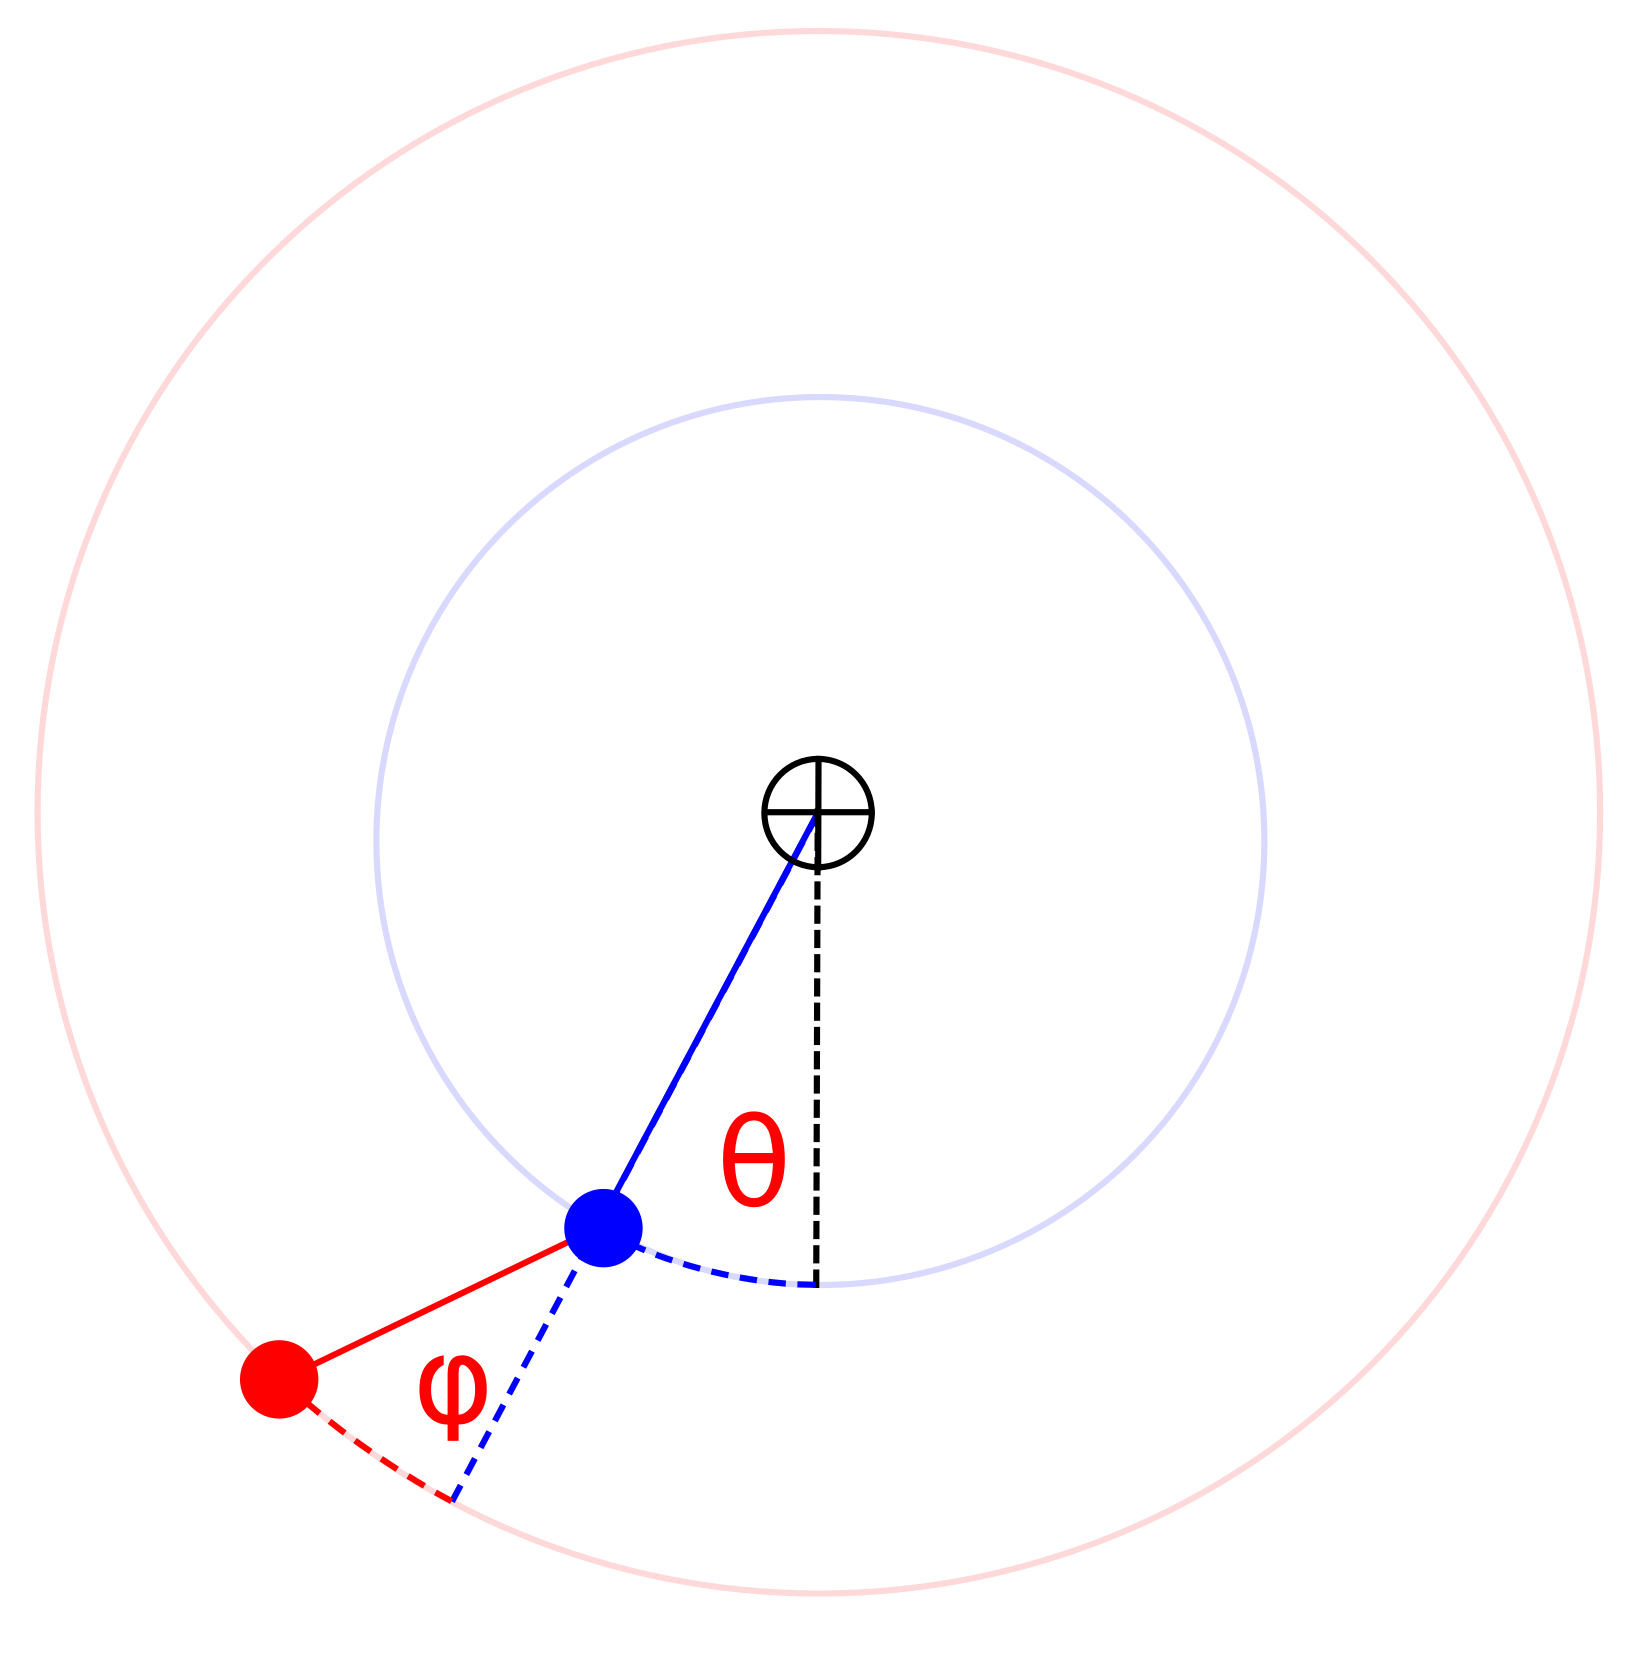
\includegraphics[width=.75\textwidth]{Pictures/bipend-abstract}	
				\end{center}
			\end{column}
			\begin{column}{0.5\textwidth}
				\begin{center}
					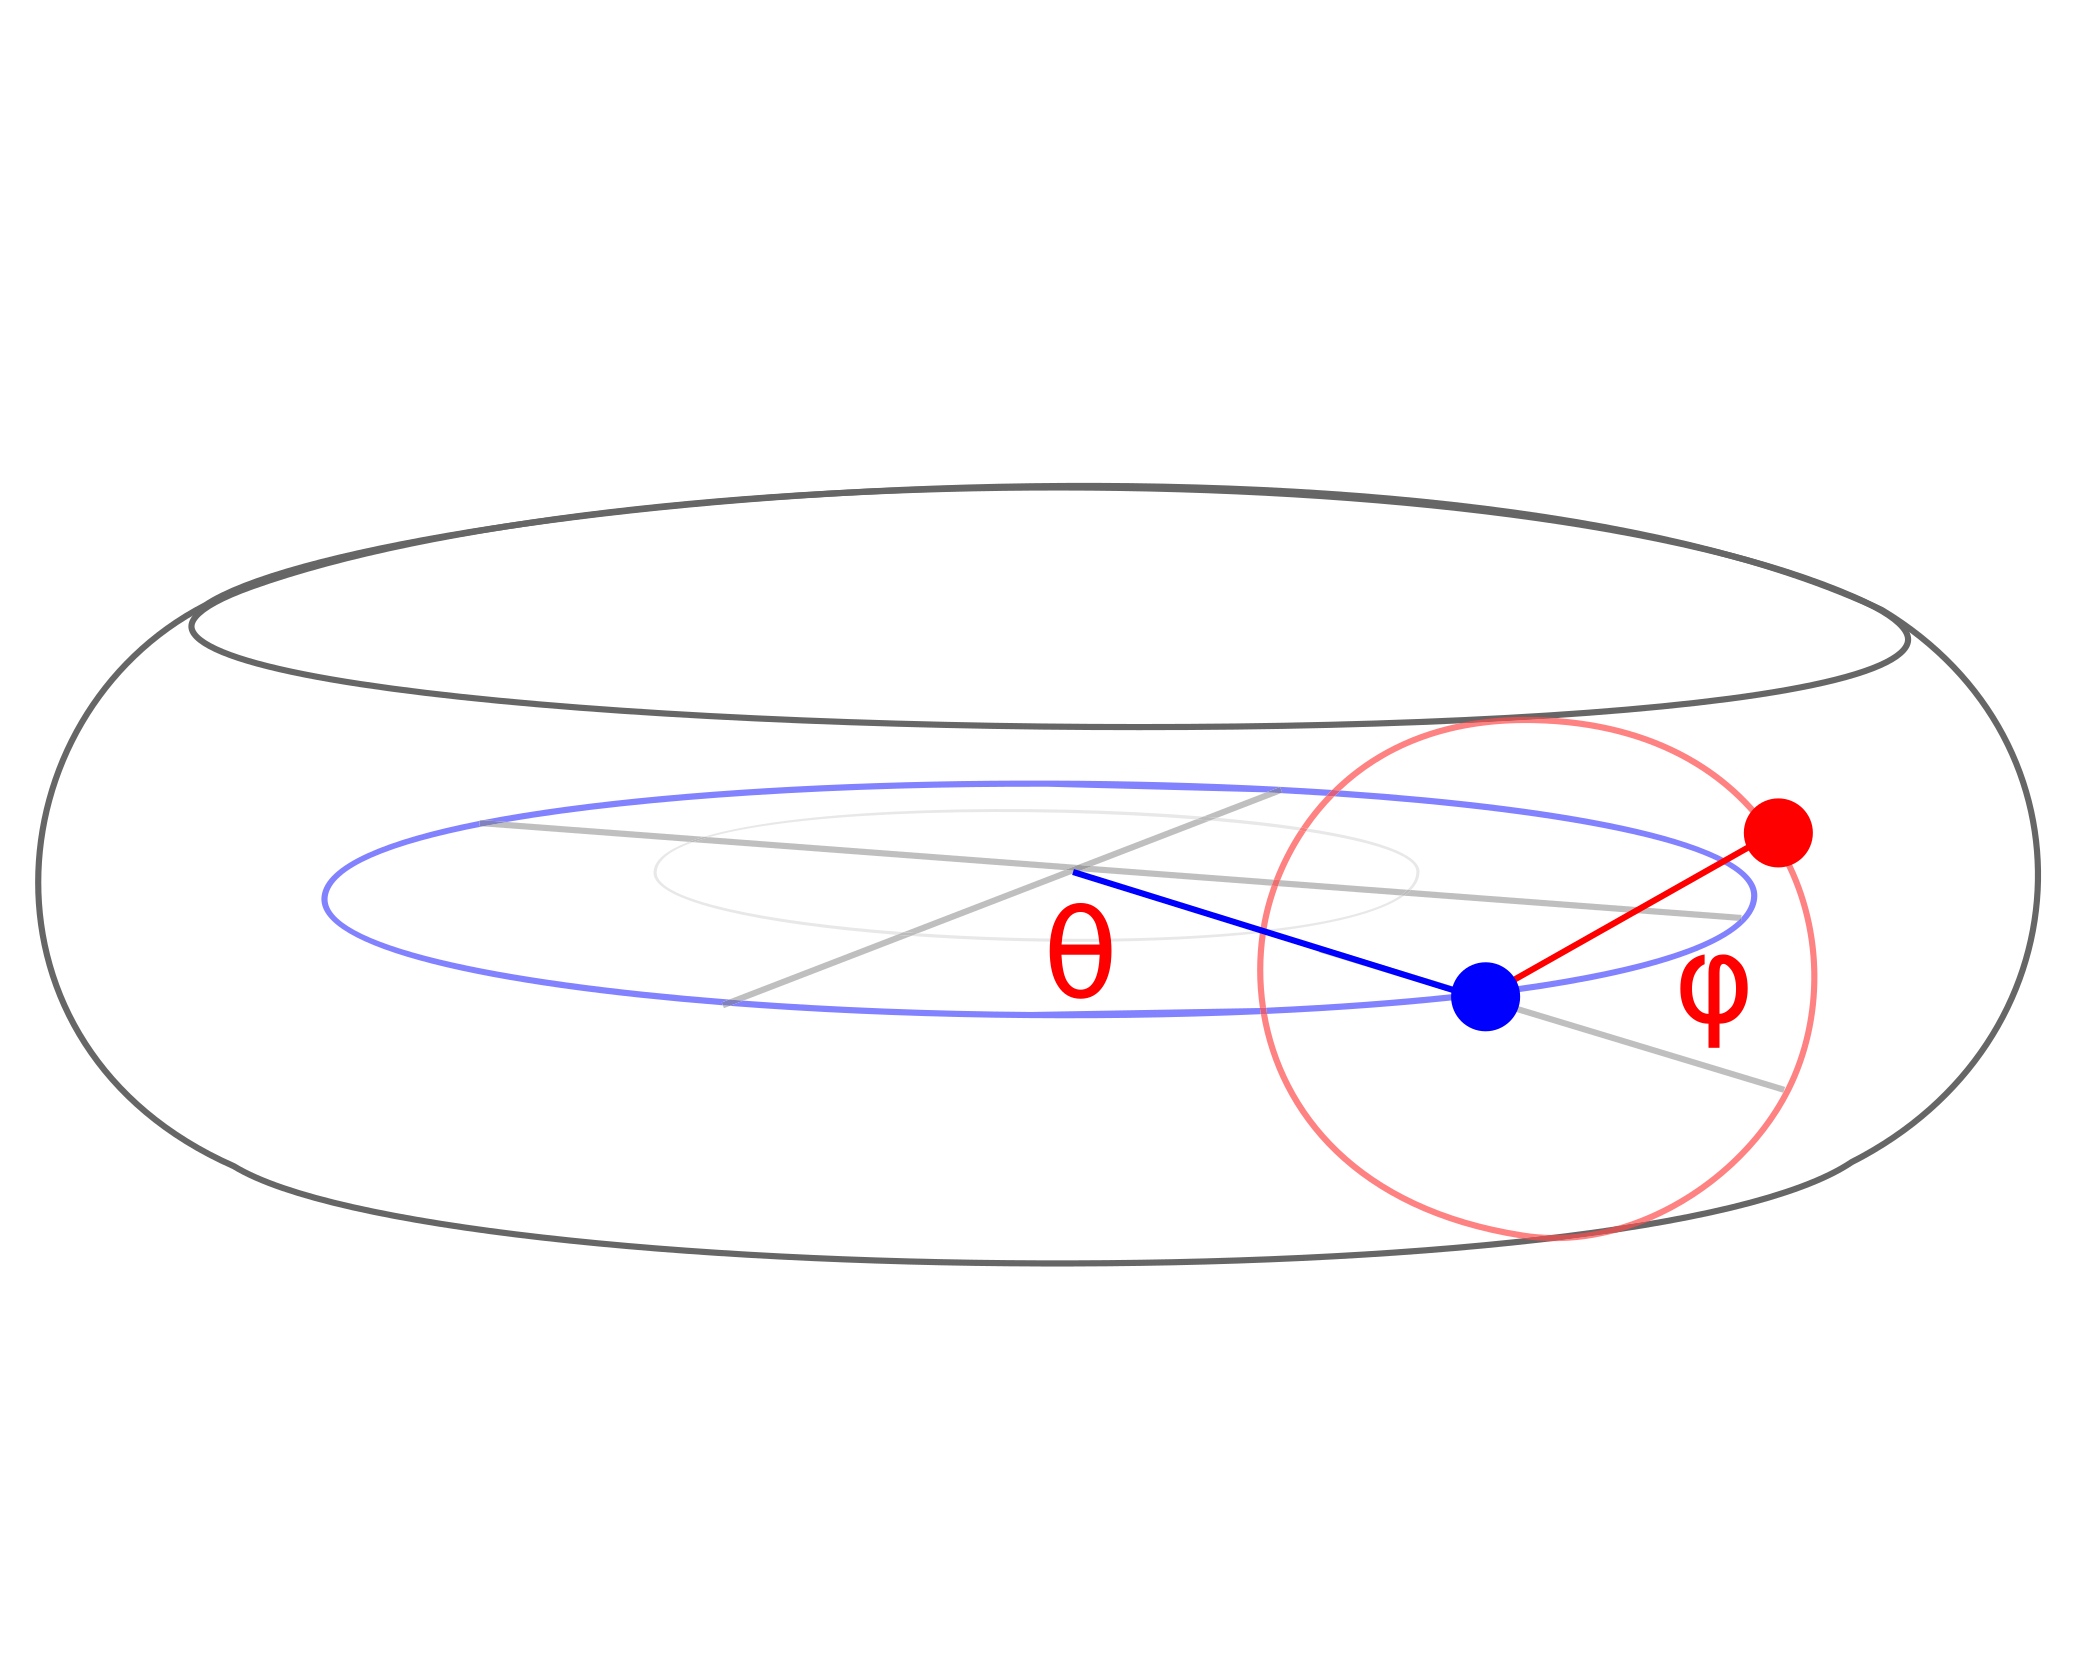
\includegraphics[width=.75\textwidth]{Pictures/bipend-phase}	
					\alert{Configuration space is a Torus}
				\end{center}
			\end{column}
		\end{columns}	
	
\end{frame}
\note[itemize]{
	\item \animategraphics[autoplay,palindrome,width=\textwidth]{5}{Pictures/lessig-pibend-frame/bipend-}{2}{6}
	\item This case (bi-pendulum) exemplify how constraints can be enforced intrinsically choosing an appropriate geometric framework. (2-coordinates instead of the 4 x-y coordinates needed to fix the two endpoints.
		\item Although it is a toy model it is the first step in modelling a protein. (Chain of amino acids placed at almost constant distance between them)
}
\else
\begin{frame}[t]{Configuration Space: a slightly more difficult example}
		\center
	\begin{bracketbox}
		Double pendulum.
	\end{bracketbox}
	

	\vfill
	\only<1-3>{
		\begin{columns}[T]
			\begin{column}{0.5\textwidth}
				\begin{center}
					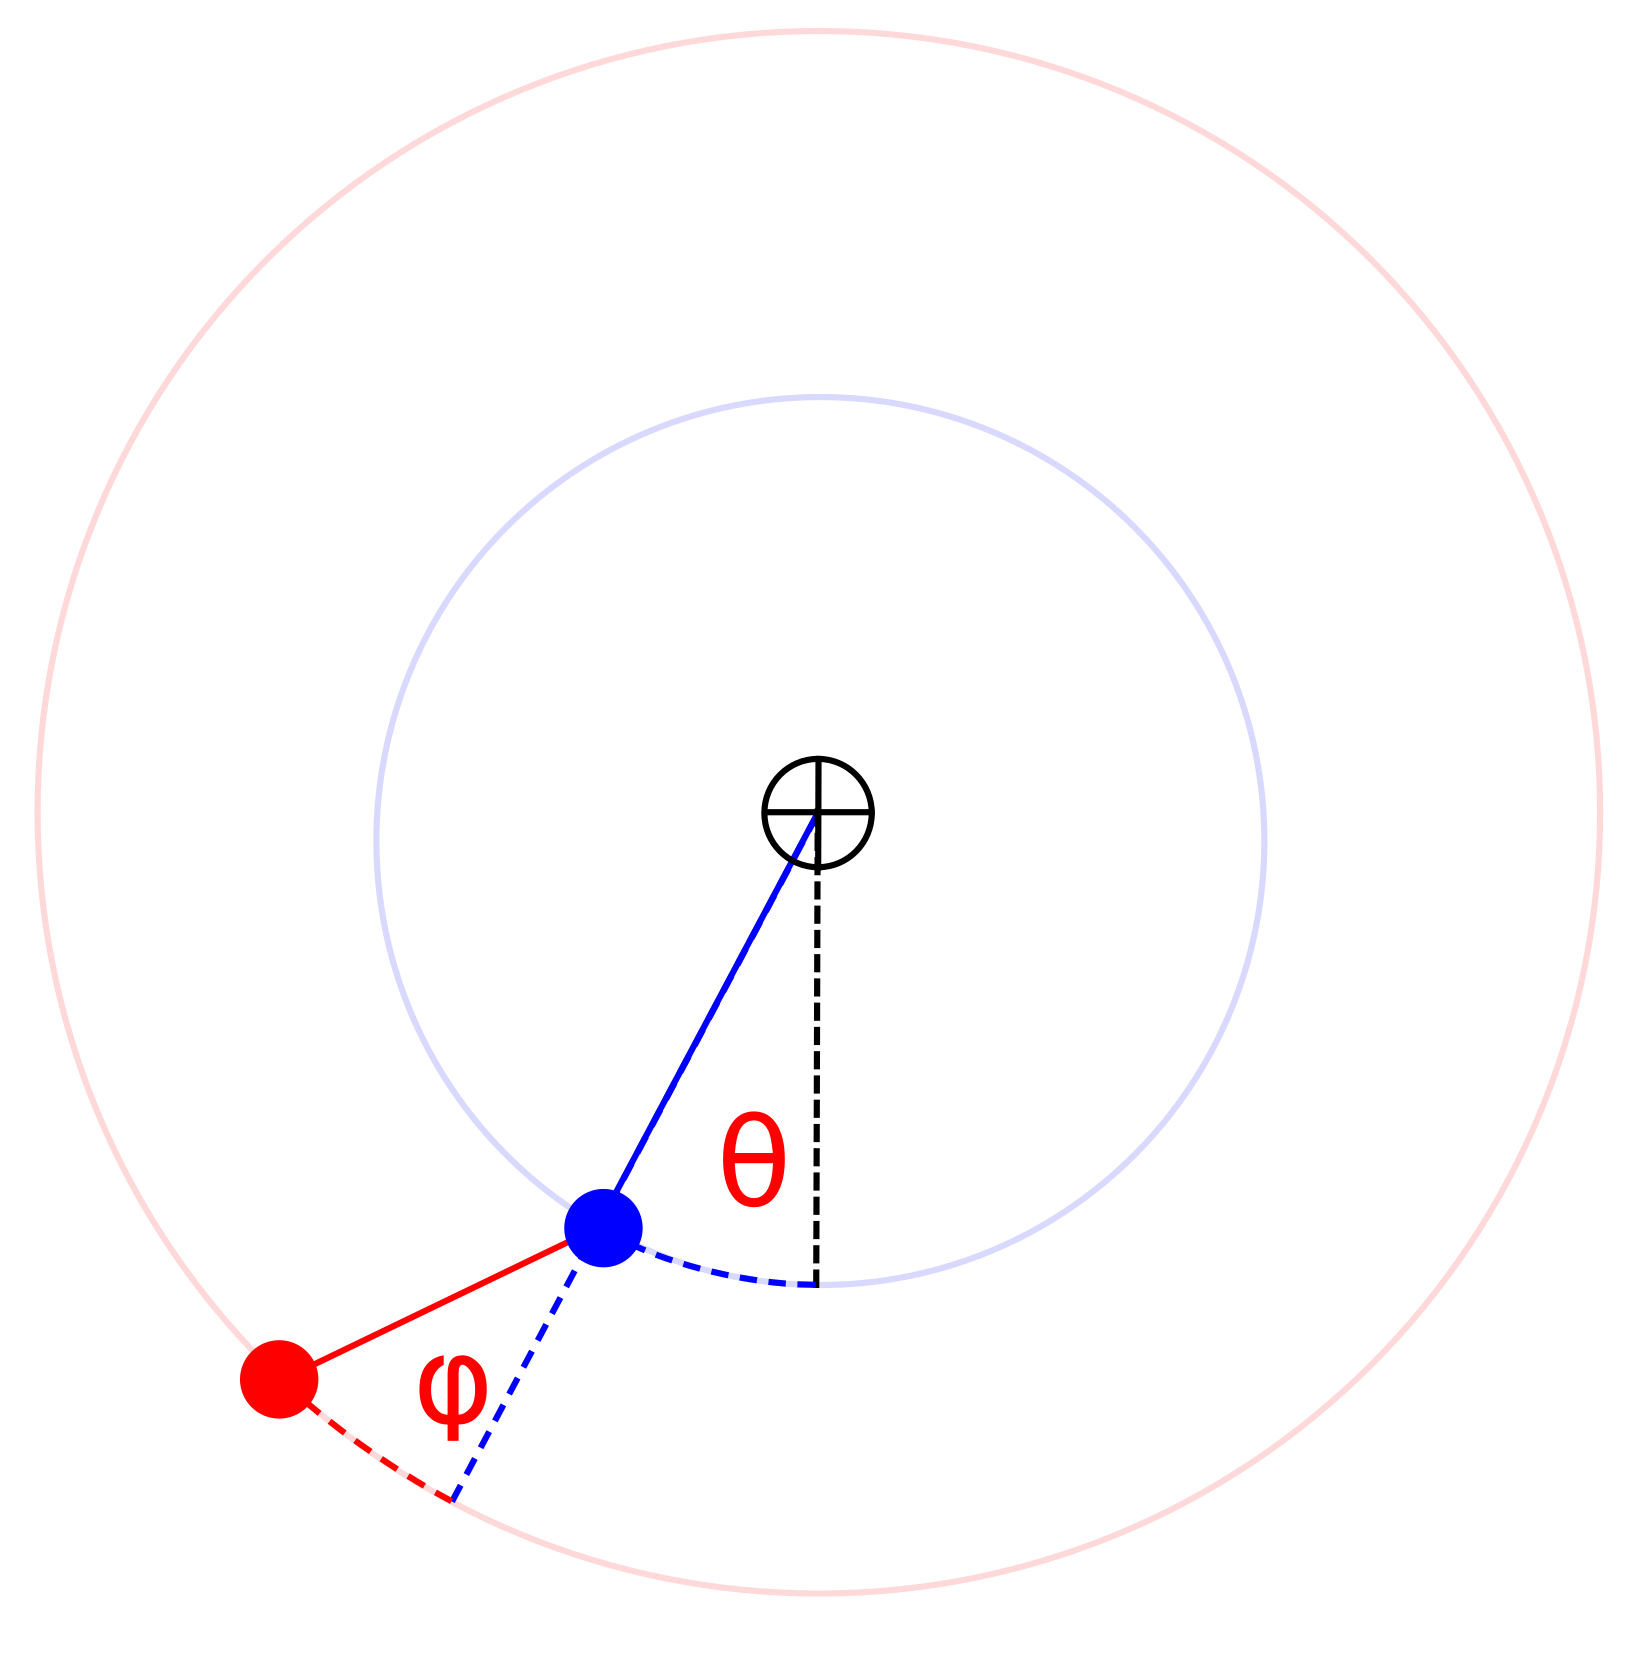
\includegraphics[width=.75\textwidth]{Pictures/bipend-abstract}	
				\end{center}
			\end{column}
			\begin{column}{0.5\textwidth}
				\begin{center}
					\only<1>{
						\noindent Toy model for:
						\begin{center}
							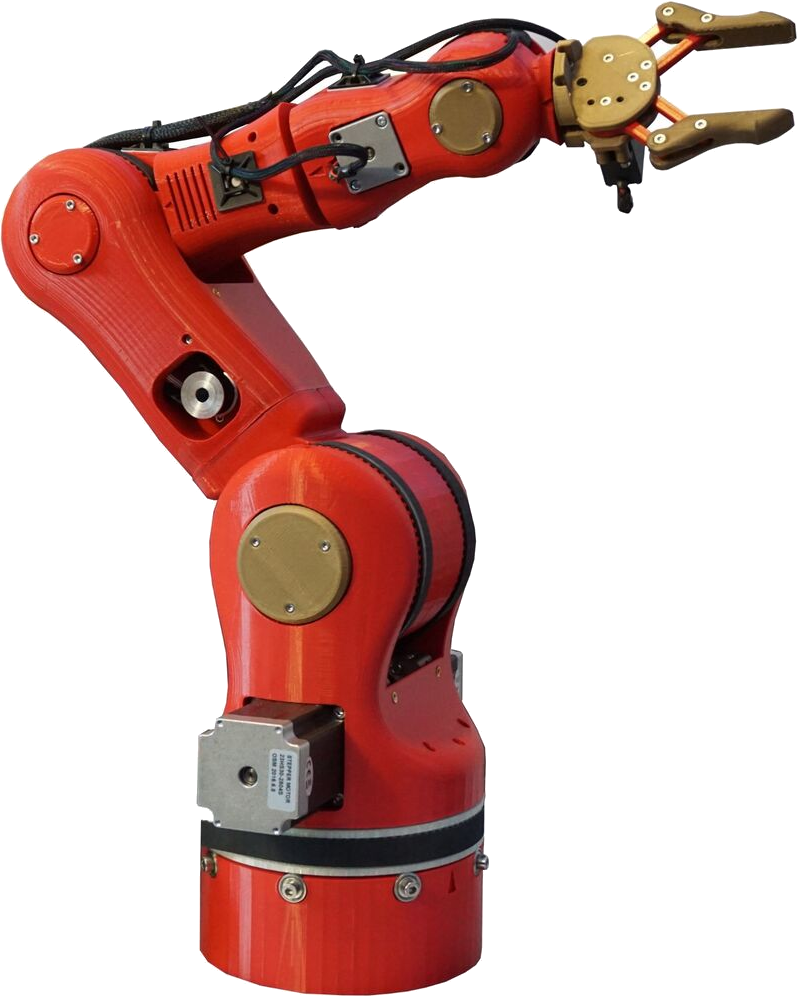
\includegraphics[width=.55\textwidth]{Pictures/robo_arm}
						\end{center}
						mechanical arms.
					}
					\only<2>{
						\noindent Toy model for:
						\begin{center}
							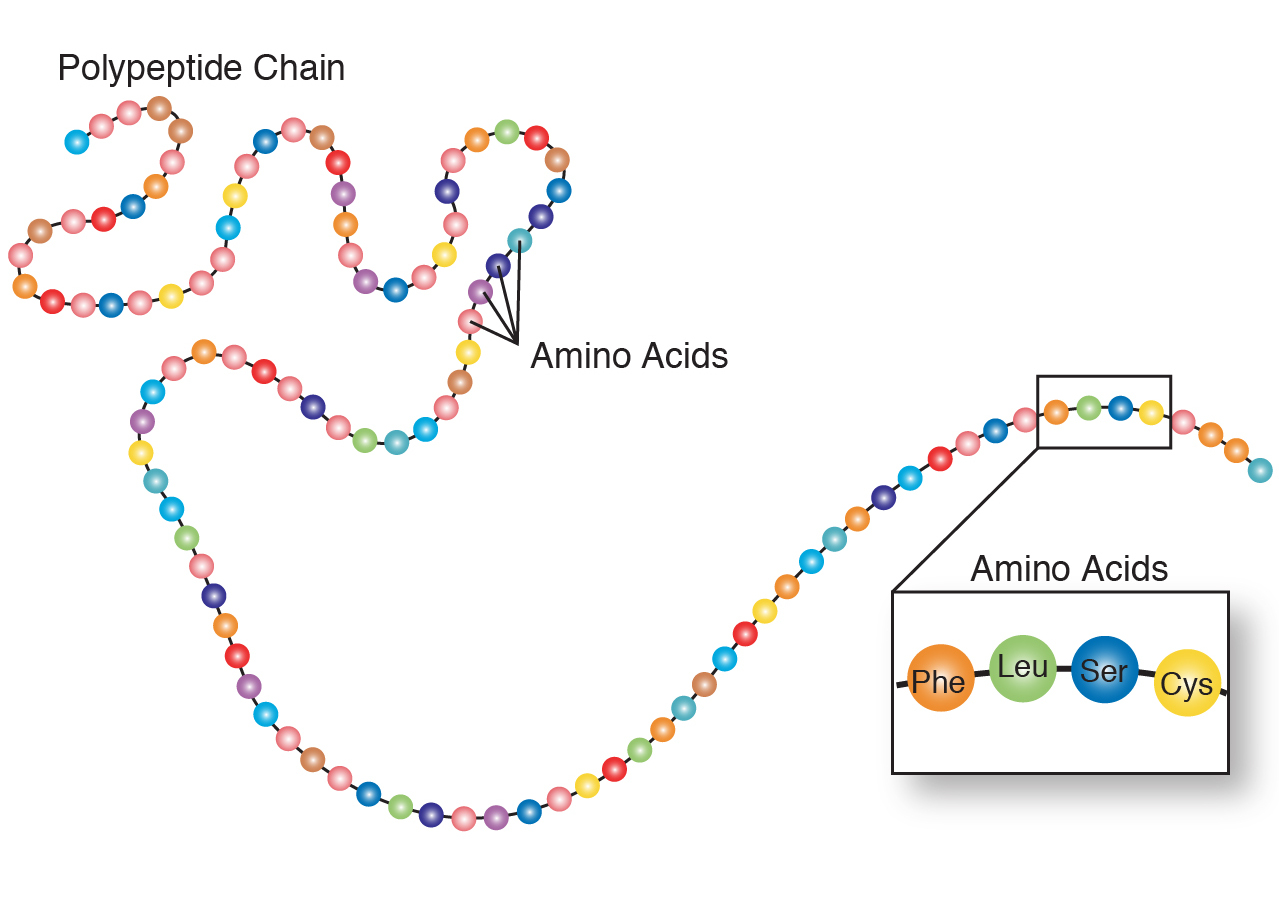
\includegraphics[width=.65\textwidth]{Pictures/amino_acids}
						\end{center}
						Proteins (amino acid chains).	
					
					}
					\only<3>{
						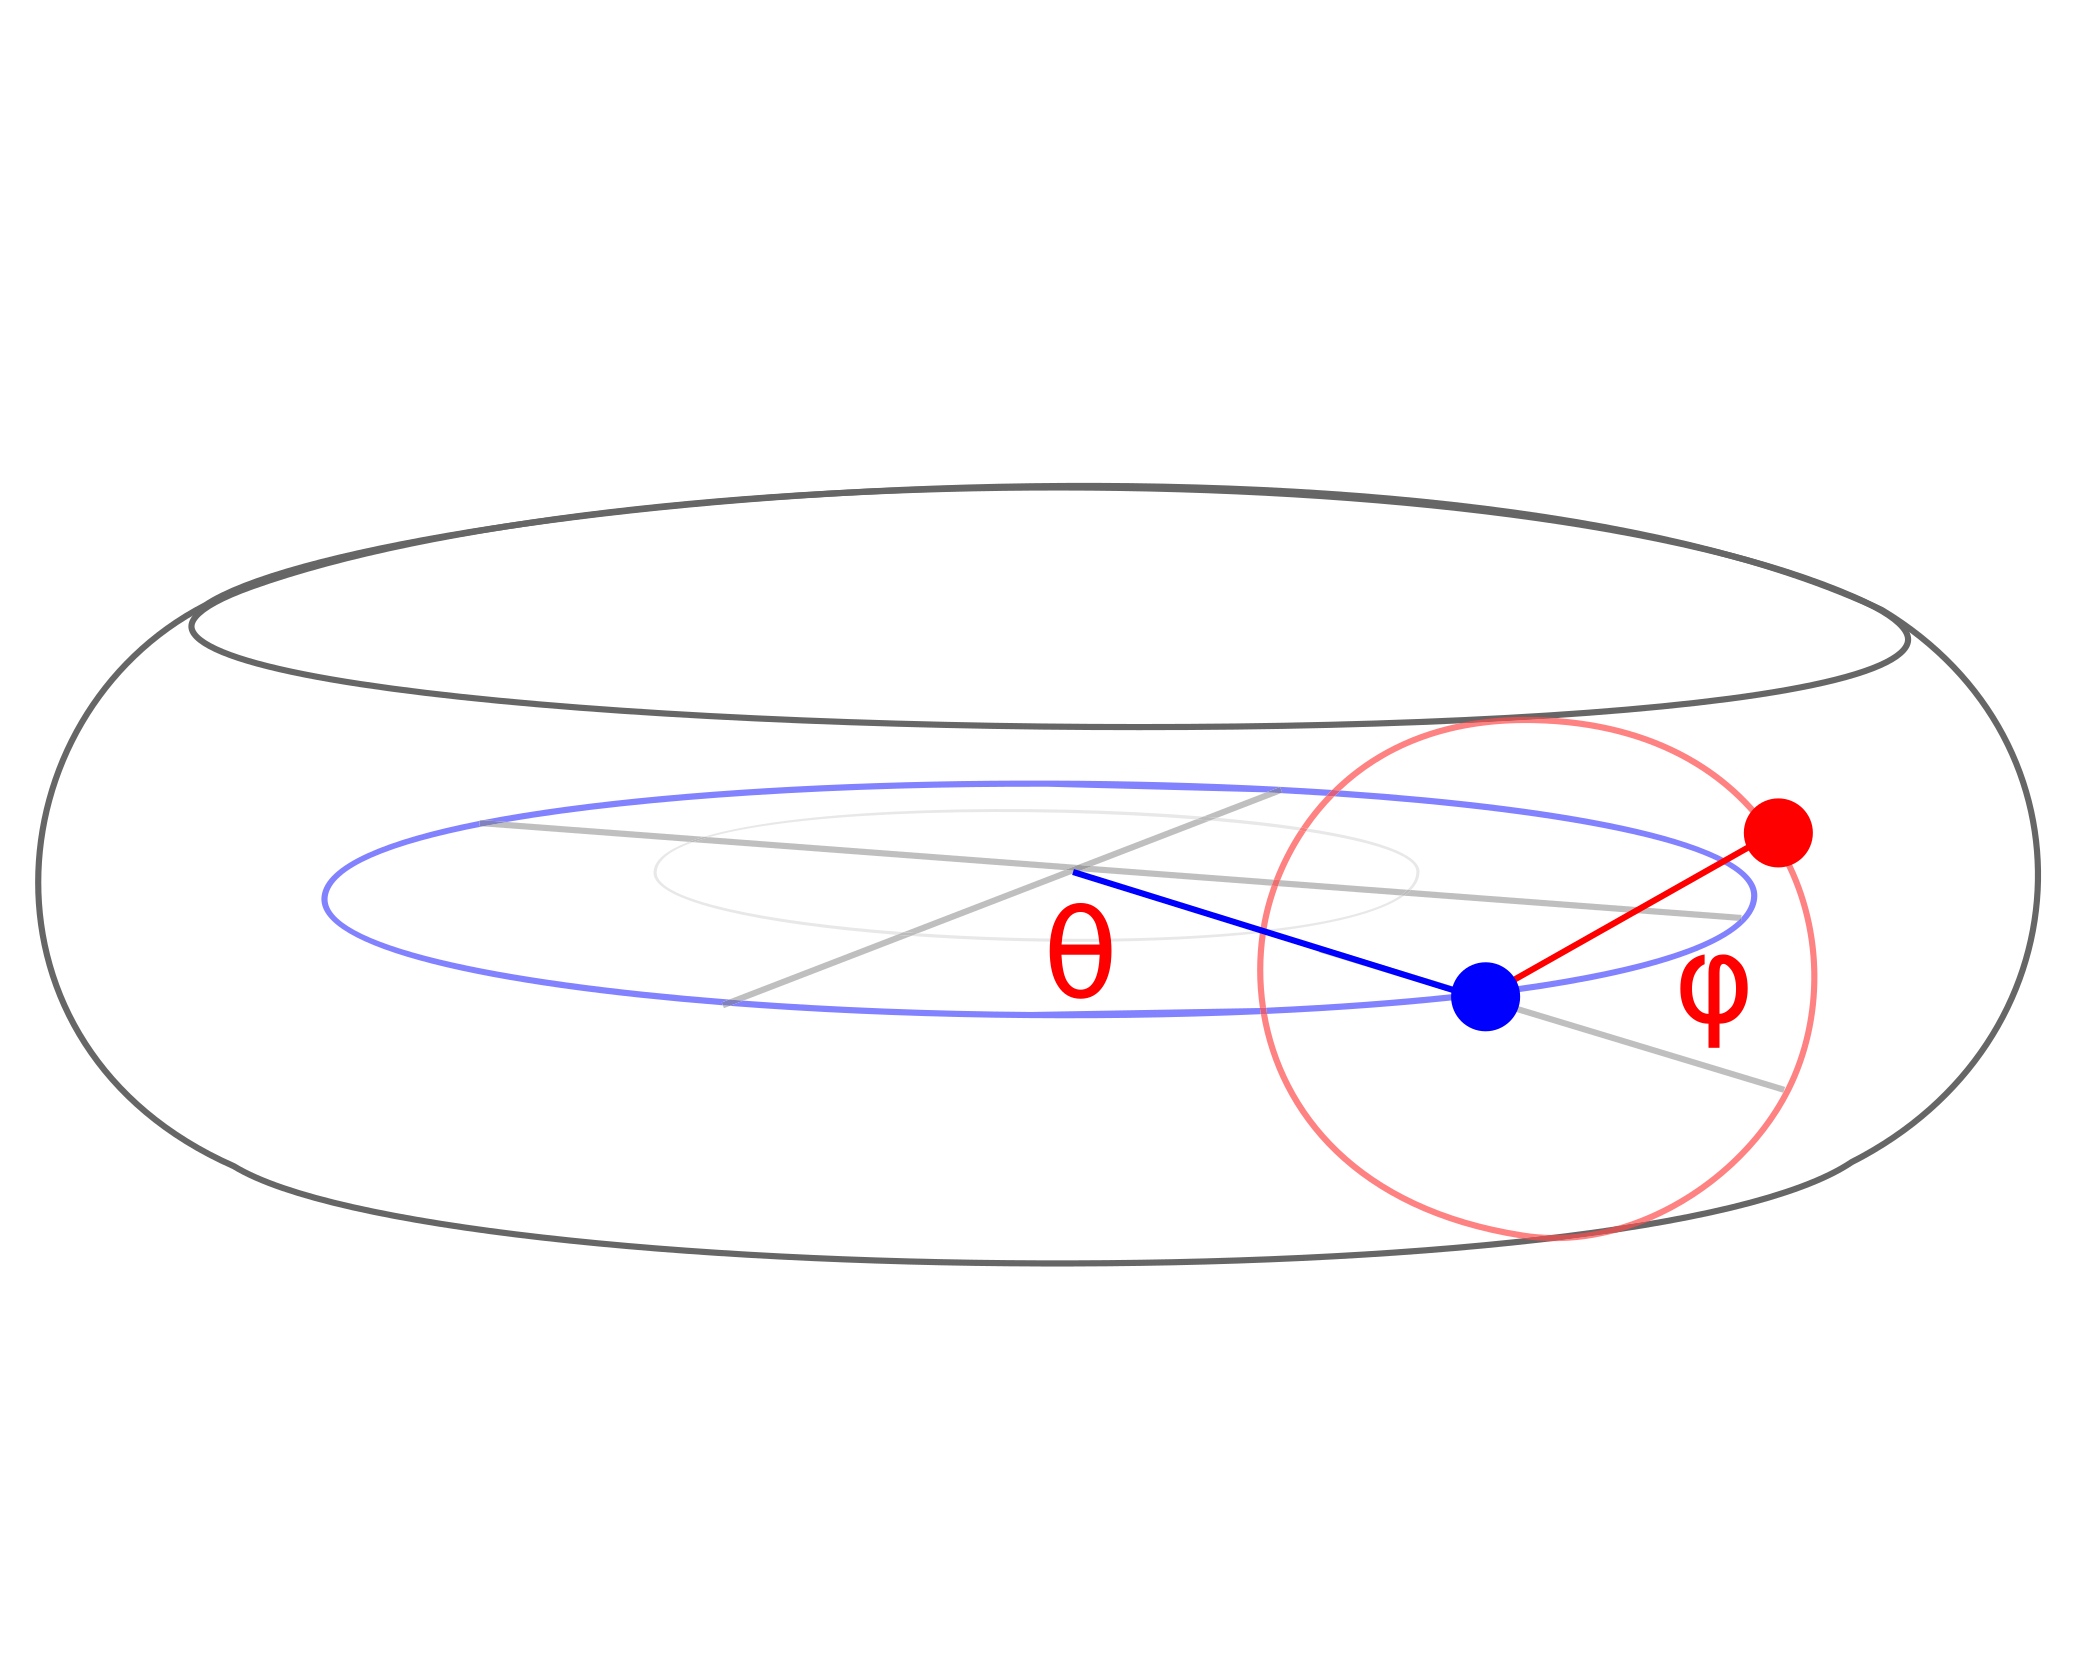
\includegraphics[width=.75\textwidth]{Pictures/bipend-phase}	
					}
				\end{center}
			\end{column}
		\end{columns}	
	}
	\only<4->{
		\animategraphics[autoplay,palindrome,width=\textwidth]{5}{Pictures/lessig-pibend-frame/bipend-}{2}{6}
	}
	\vfill
	\onslide<3->{\center\alert{Configuration space is a Torus}}


\end{frame}
\fi
%-------------------------------------------------------------------------------------------------------------------------------------------------

\end{document}